\section{Experimental Results}
\label{chap:results}

%===============================================================
\subsection{Baseline Inference}
%===============================================================

In Fig.~\ref{fig:untuned_samples} we can see that the unmodified AutoBrep model indeed generates impressive B-Rep's with high complexity and apparent correctness. Each of these STEP samples were rendered from various angles and concatenated in a GIF showing them from all directions for inspection.

\begin{figure}[h!]
	\centering
	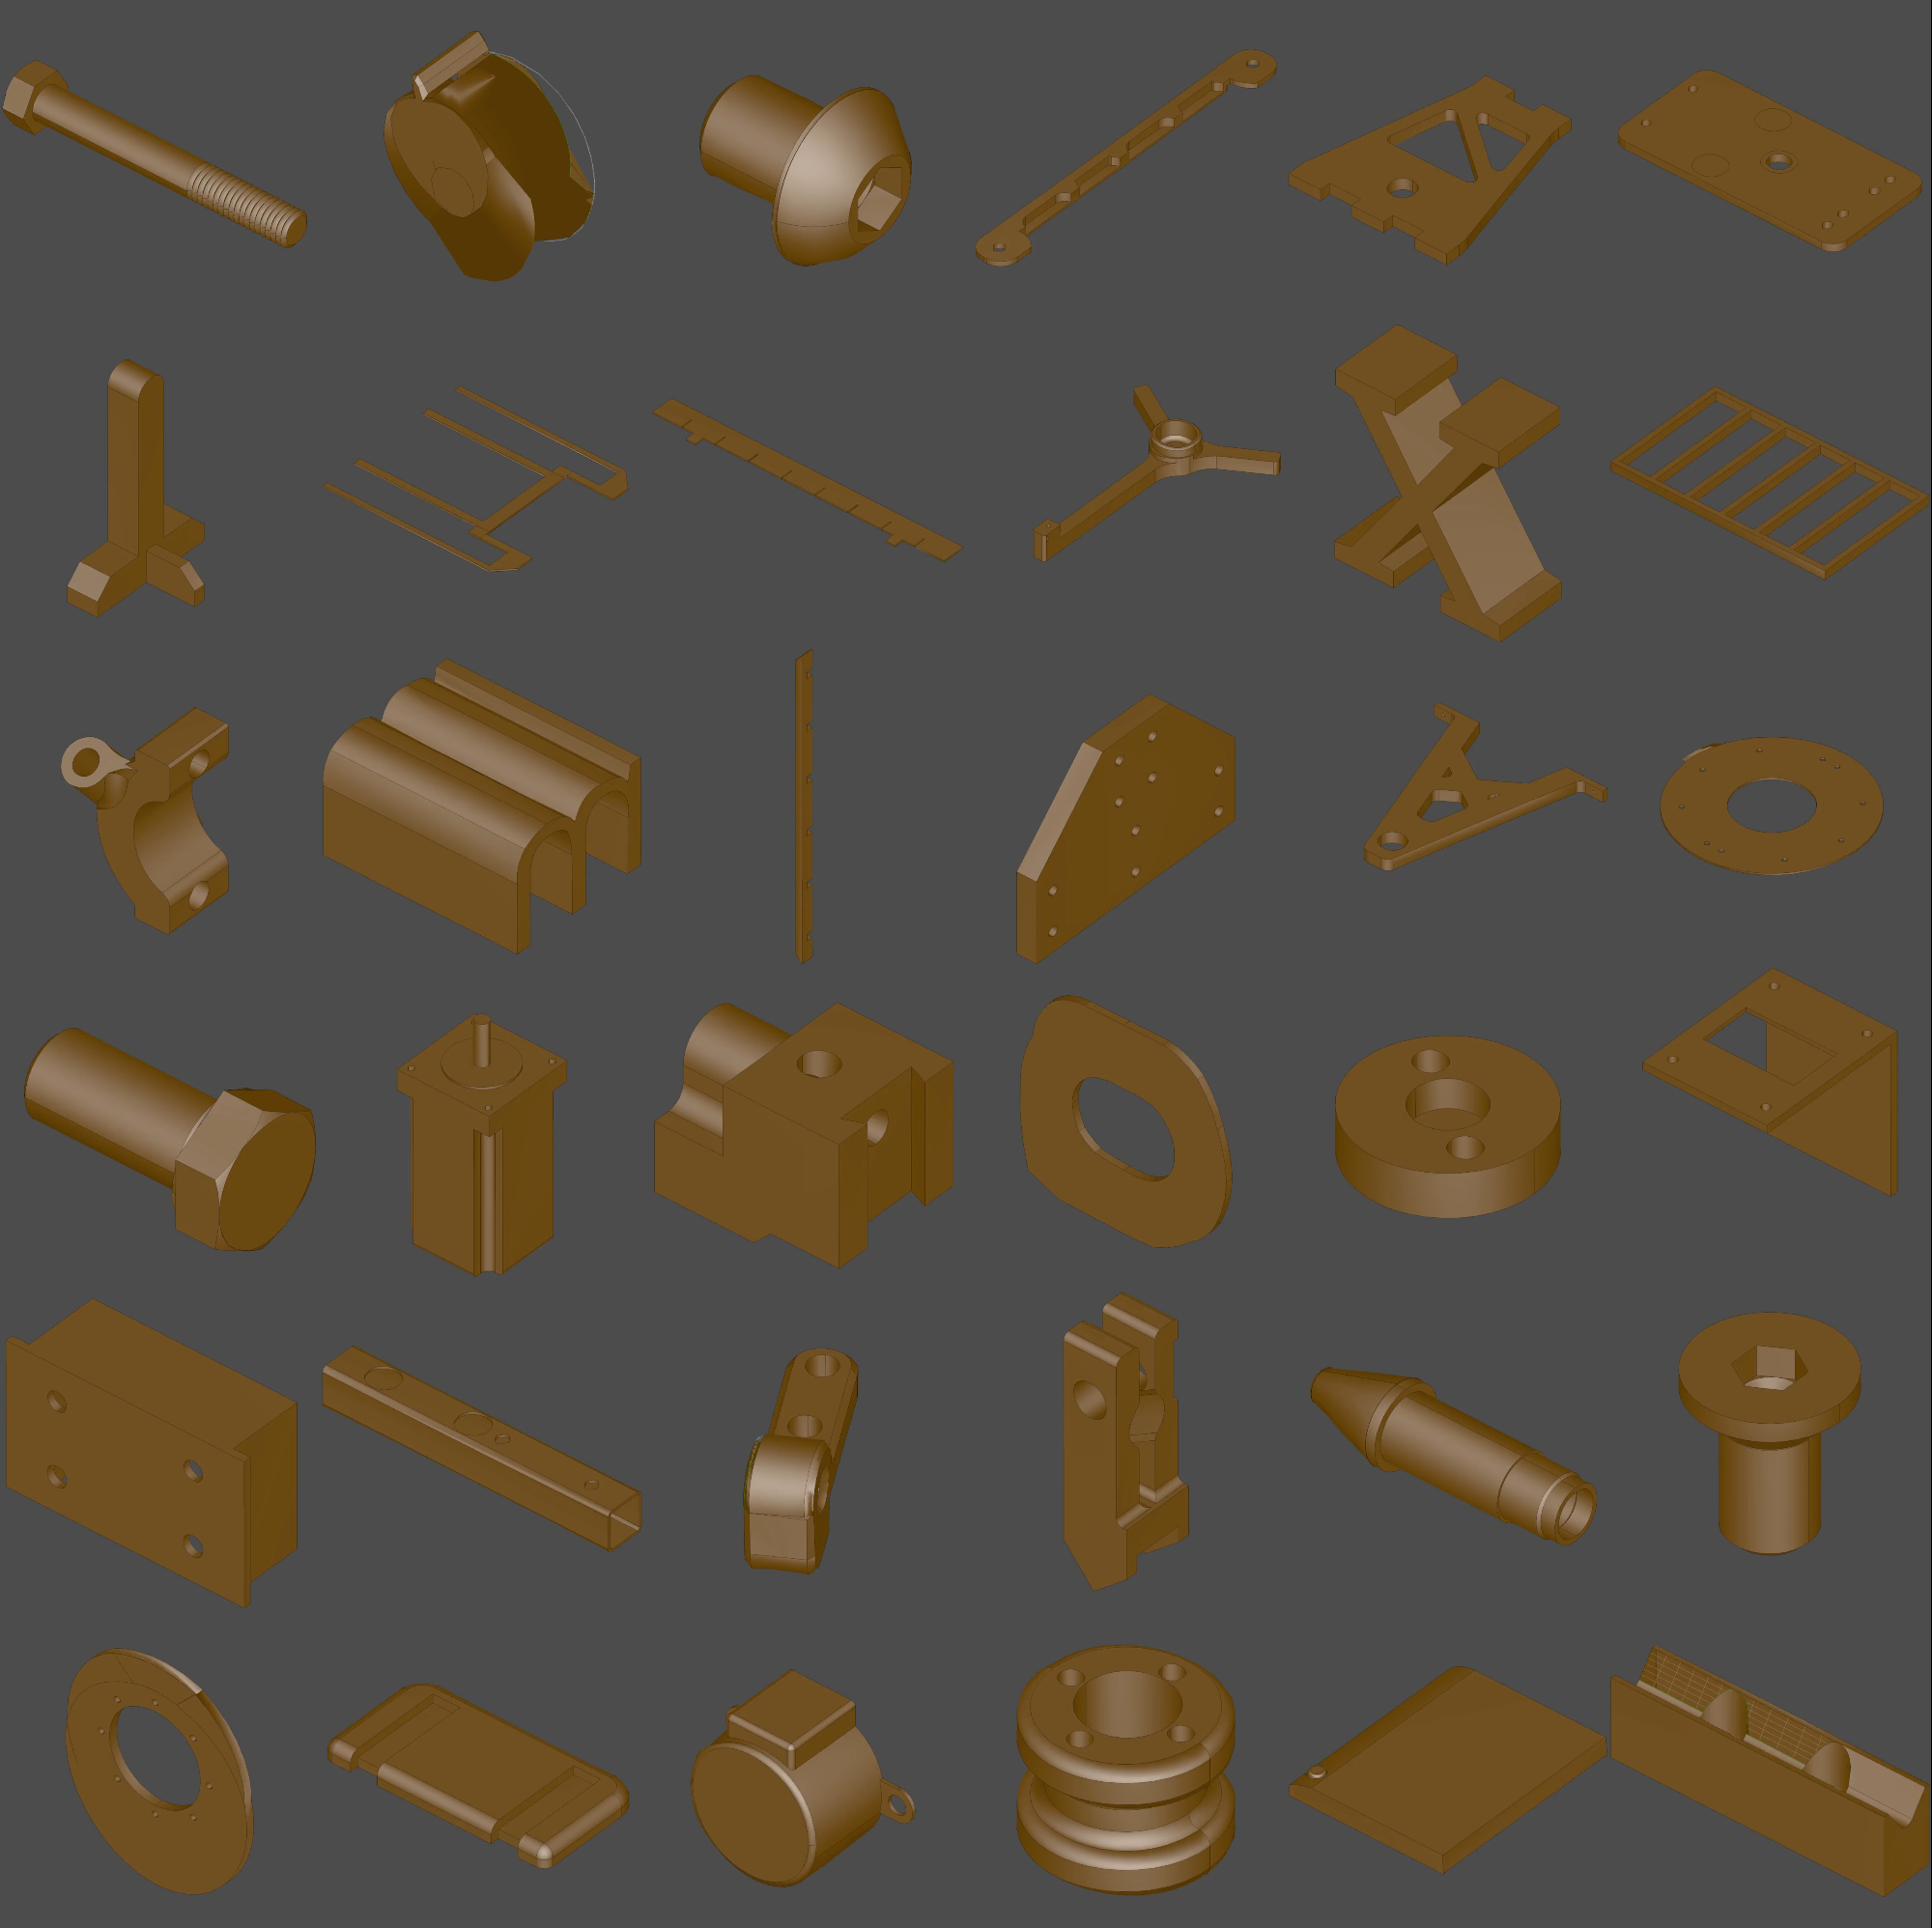
\includegraphics[width=0.66\textwidth]{figures/untuned_medium.png}
	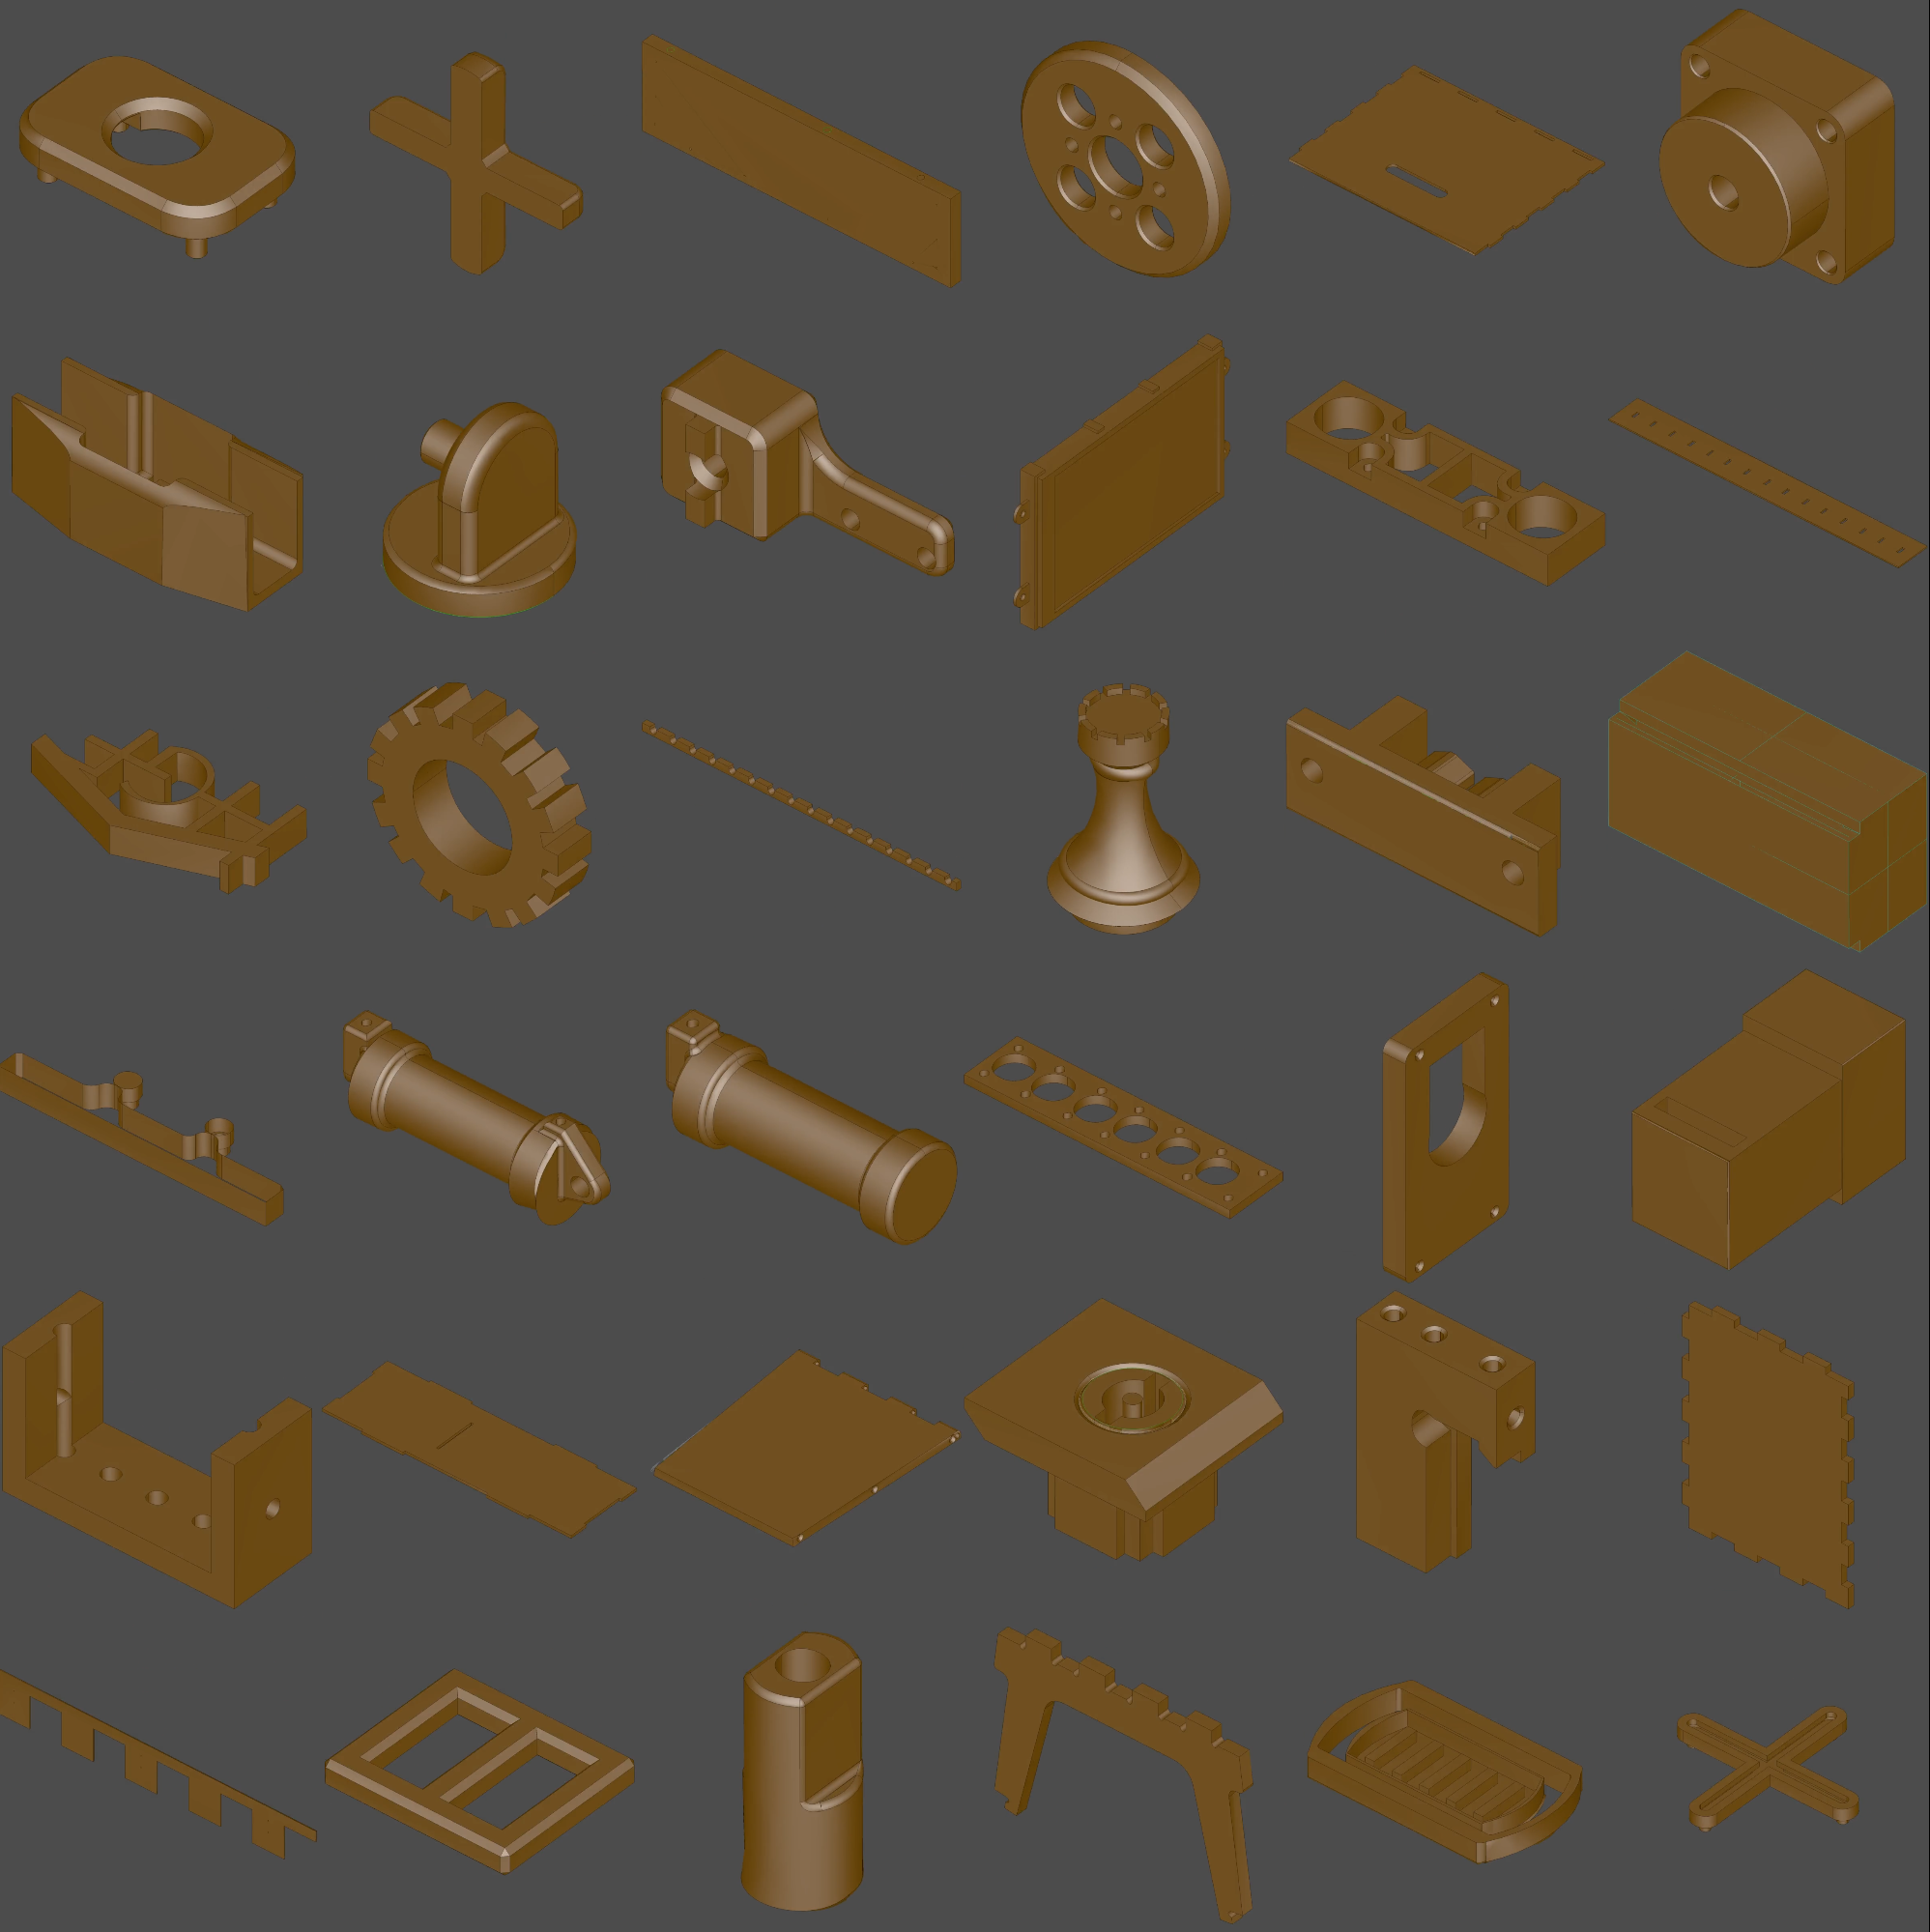
\includegraphics[width=0.66\textwidth]{figures/untuned_hard.png}
	\caption{Examples of unconditional samples generated with the untuned base model checkpoint. Top with medium complexity (25 to 50 faces per shape) and bottom with high complexity (50+ faces per shape).}
	\label{fig:untuned_samples}
\end{figure}

Generated models demonstrate:
\begin{itemize}
	\item \textbf{Geometric Validity}: Faces and edges form coherent solid structures
	\item \textbf{Diversity}: Multiple samples exhibit varied feature combinations
	\item \textbf{Domain Adherence}: Generated geometry aligns with training domain characteristics
\end{itemize}

%===============================================================
\subsubsection{Comparison with BrepGen}
%===============================================================

To contextualize AutoBrep's performance, we compare it with BrepGen, the predecessor diffusion-based approach discussed in Chapter~\ref{chap:background}. Figure~\ref{fig:brepgen_samples} shows representative samples generated with BrepGen.

\begin{figure}[h!]
	\centering
	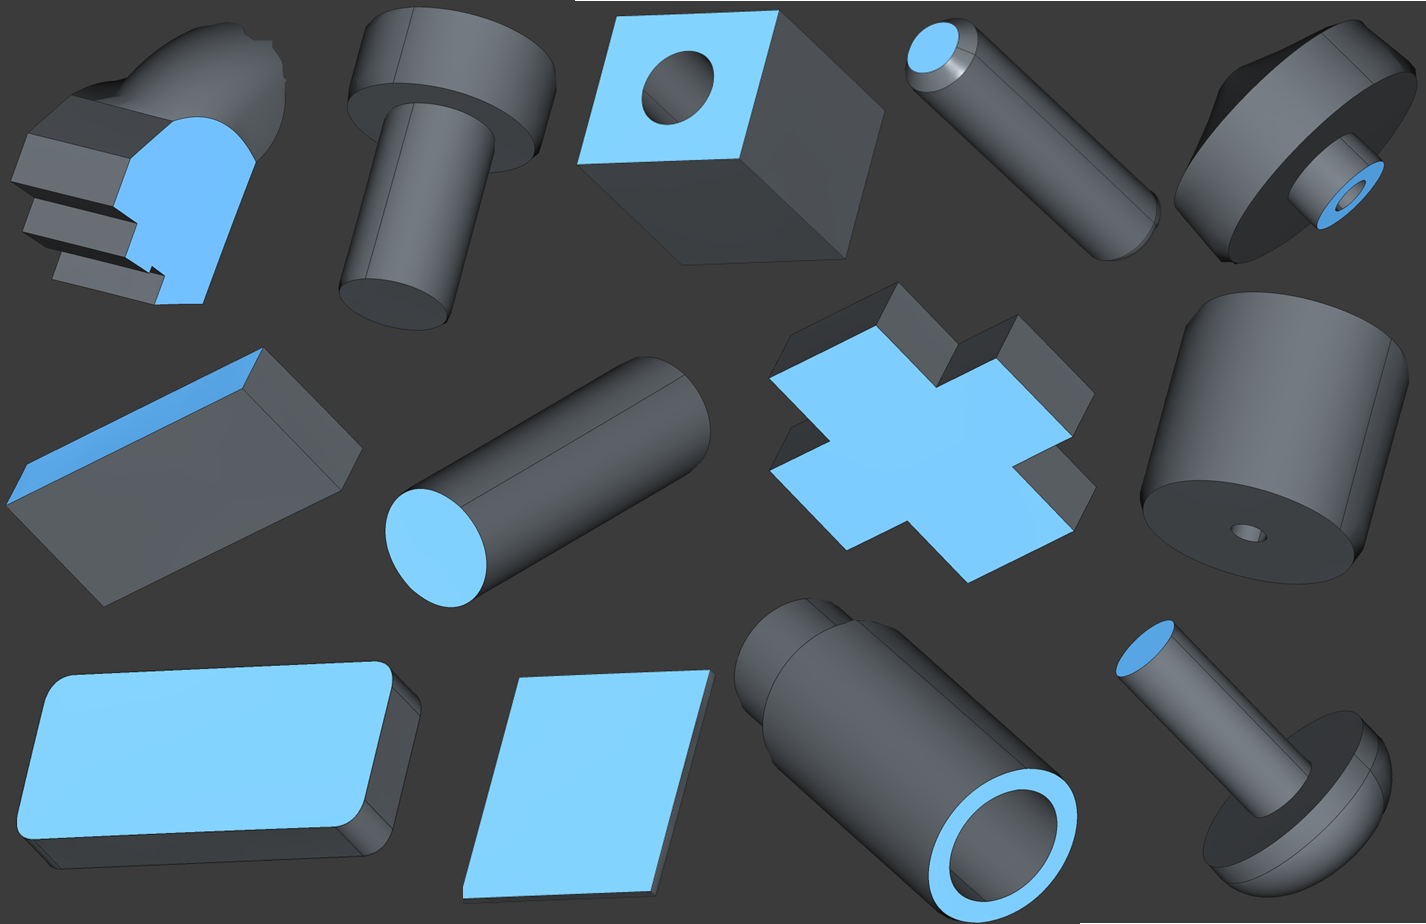
\includegraphics[width=0.66\textwidth]{figures/BrepGen.png}
	\caption{Representative samples generated with BrepGen (diffusion-based approach) from unconditional generation. While geometrically valid, BrepGen produces predominantly simple geometries with low complexity: mainly cylinders and cuboids with chamfers and holes. This limitation in generated geometric diversity motivated the selection of AutoBrep, which generates higher-complexity solids with more varied topological structures.}
	\label{fig:brepgen_samples}
\end{figure}

AutoBrep offers several key advantages over BrepGen: higher geometric complexity with diverse topological structures versus BrepGen's simple geometries (cylinders, cuboids with chamfers and holes), superior feature diversity across complexity ranges, 2--5$\times$ faster generation speed through single-stage autoregression, and better scalability supporting up to 100+ face solids.

\textbf{Base Model Constraints:} During baseline inference evaluation, we observed that the unconditionally-trained base model does not support conditional generation tasks such as autocomplete or sequence completion. The provided checkpoint appears to have been trained without geometry tokens (which are commented out in the repository code), limiting its ability to complete partial B-Rep sequences.


%===============================================================
\subsection{Training Convergence}
%===============================================================

The LoRA fine-tuning process was conducted on custom CAD model datasets, following the training setup and hyperparameters specified in Chapter~\ref{chap:methodology}.

\textbf{Training Strategy:} A key finding was that maintaining validation loss close to training loss was essential for avoiding both underfitting and overfitting. This was achieved by targeting a training loss of approximately 1.0, which empirically provided the optimal balance.

\textbf{Observed Training Characteristics:}
\begin{itemize}
	\item Training loss consistently converged toward target of 1.0 within 3--7 epochs across all datasets tested
	\item Validation loss tracked closely with training loss when hyperparameters were properly tuned (typically within 10--20\% separation)
	\item Learning rate emerged as the dominant control parameter: too high rates ($> 1 \times 10^{-4}$) caused rapid overfitting with near-zero training loss and degenerate model outputs
	\item LoRA rank and temperature had minimal influence on training convergence dynamics
	\item Gradient accumulation and bfloat16 casting proved sufficient for training on single GPU without memory issues
\end{itemize}

Training and validation loss curves are shown in Fig.~\ref{fig:training_loss}.

\begin{figure}[h!]
	\centering
	\fbox{\texttt{[Insert training/validation loss curves from W\&B export]}}
	\caption{Training and Validation Loss Over Epochs for Representative LoRA Fine-Tuning Run. Model converges toward target loss of 1.0, with validation loss tracking training loss closely.}
	\label{fig:training_loss}
\end{figure}

%===============================================================
\subsection{Empirical Findings on LoRA Fine-Tuning Dynamics}
\label{sec:lora_dynamics}
%===============================================================

\textbf{LoRA Behavior as Distribution Sharpener:} Through systematic experimentation, LoRA was observed to function as a \emph{distribution sharpener} rather than a distribution shifter. When applied to attention layers alone, LoRA concentrates probability mass on modes already present in the base model's feature space, but cannot learn genuinely novel geometric features outside this space. This fundamentally constrains what fine-tuning can achieve: the base model must already contain (in distributed form) the geometric features present in the fine-tuning data.

\textbf{Effect of Adapter Placement:} Experiments comparing attention-only adapters (as specified in Chapter~\ref{chap:methodology}, Table~\ref{tab:lora_params}) with attention + feed-forward adapters revealed minimal differences in output quality or decodability. Figure~\ref{fig:lora_adapters_comparison} illustrates the marginal improvement from adding feed-forward adapters. This finding supports the hypothesis that most adaptation occurs through attention weight redistribution, with feed-forward layers providing limited additional benefit.

\begin{figure}[h!]
	\centering
	\fbox{\texttt{[Insert comparison: attention-only LoRA vs. attention+FF LoRA at T=0.6]}}
	\caption{LoRA Adapter Configuration Comparison. Left: attention-only adapters. Right: attention + feed-forward adapters. Addition of FF adapters provides minimal visible improvement in output quality or diversity.}
	\label{fig:lora_adapters_comparison}
\end{figure}

%===============================================================
\subsection{Quantitative Evaluation}
%===============================================================

\textbf{Model Quality Metrics:} Model performance is assessed through multiple quantitative measures derived from training and inference experiments.

\textbf{Decodability Rate:} A critical metric for generative B-Rep models is the fraction of generated sequences that successfully decode into valid solids. Across all fine-tuning runs, the fine-tuned LoRA models achieved approximately 90\% decodability rate under normal inference conditions (temperature $T \in [0.5, 0.8]$). This rate remained high unless the model exhibited signs of overfitting (near-zero training loss due to excessive learning rate or epoch count), in which case generated sequences became degenerate and decoding failed completely.

\textbf{Temperature Sensitivity:} Inference temperature was varied across the range $T \in [0.3, 0.8]$ to assess its impact on output diversity and fidelity to training data. Key findings:

\begin{itemize}
	\item \textbf{Low temperature ($T \approx 0.3$)}: Model outputs concentrated on the most probable modes, with minimal diversity. Strong LoRA effect.
	\item \textbf{Optimal range ($T \in [0.5, 0.7]$)}: Best balance between resemblance to training data and geometric diversity. Results showed prominent training features (e.g., holes, cylinders, cubes) but not exact reproductions of training shapes.
	\item \textbf{High temperature ($T > 0.8$)}: Increased diversity but reduced fidelity to training distribution. Model samples from broader set of modes beyond training data.
\end{itemize}

Temperature had minimal impact on decoding success rate; failures were primarily driven by model overfitting rather than inference temperature.

\textbf{Loss Metrics:} Validation loss provided the primary signal for hyperparameter tuning. The strategy of targeting training loss $\approx 1.0$ successfully maintained reasonable separation between train and validation curves, with typical validation loss within 10--20\% of training loss for well-tuned models.

Further evaluation against baseline (untuned AutoBrep) is presented in Section~\ref{sec:ablation}.

%===============================================================
\subsection{Qualitative Results}
%===============================================================

Generated B-Reps are visualized and evaluated for geometric plausibility, feature fidelity, and diversity relative to training data.

\textbf{Cylinders with Holes Dataset:} Fine-tuning was performed on 600 cylindrical solids with through-holes. The fine-tuned model produced results featuring:

\begin{itemize}
	\item Cylindrical geometry (primary feature)
	\item Through-holes positioned and sized in plausible locations
	\item Variations in hole placement and size
	\item Decodable, watertight solids in approximately 90\% of samples
\end{itemize}

Examples are shown in Fig.~\ref{fig:cylinders_results}.

\begin{figure}[h!]
	\centering
	\fbox{\texttt{[Insert 3 representative cylinder-with-holes samples at T=0.6]}}
	\caption{Qualitative Results: Cylinders with Holes. Fine-tuned LoRA model generates cylindrical solids with through-holes. While not exact reproductions of training data, samples exhibit characteristic training features (cylindrical body, hole placement).}
	\label{fig:cylinders_results}
\end{figure}

\textbf{Cubes with Holes Dataset:} Fine-tuning was also performed on 600 cubic solids with holes, producing analogous results:

\begin{itemize}
	\item Cubic or near-cubic primary geometry
	\item Through-holes with varied placement patterns
	\item High decodability (approximately 90\%)
	\item Feature amplification without exact reproduction
\end{itemize}

Examples are shown in Fig.~\ref{fig:cubes_results}.

\begin{figure}[h!]
	\centering
	\fbox{\texttt{[Insert 3 representative cube-with-holes samples at T=0.6]}}
	\caption{Qualitative Results: Cubes with Holes. Fine-tuned LoRA model generates cubic solids with through-holes. Again demonstrating feature amplification from training data.}
	\label{fig:cubes_results}
\end{figure}

\textbf{Base Model vs. LoRA Comparison:} To isolate the effect of fine-tuning, we compare unconditional samples from the base model at temperature $T=0.6$ with fine-tuned LoRA samples at the same temperature, using the same random seed for reproducibility. Figure~\ref{fig:base_vs_lora} shows this comparison.

\begin{figure}[h!]
	\centering
	\fbox{\texttt{[Insert side-by-side base model vs. LoRA samples at T=0.6]}}
	\caption{Base Model vs. LoRA Fine-Tuning. Left: unconditional samples from base AutoBrep model. Right: samples from LoRA fine-tuned on cylinders-with-holes. Note the amplification of cylindrical features in LoRA outputs.}
	\label{fig:base_vs_lora}
\end{figure}

%===============================================================
\subsection{Ablation Studies and Hyperparameter Analysis}
\label{sec:ablation}
%===============================================================

To understand the contribution of different training and inference components, systematic ablation experiments were conducted.

\textbf{LoRA Rank Impact:} Varying LoRA rank $r \in \{16, 32\}$ showed minimal influence on final output quality or convergence behavior. Both configurations achieved similar decodability rates (approximately 90\%) and produced outputs with comparable feature amplification. This suggests that the primary bottleneck is the base model's learned feature space rather than adapter capacity.

\textbf{Learning Rate Sensitivity:} Learning rate emerged as the dominant hyperparameter. The relationship was nonlinear:
\begin{itemize}
	\item Too low ($< 1 \times 10^{-5}$): Insufficient adaptation; training loss converged slowly and remained high
	\item Optimal range ($1 \times 10^{-5}$ to $1 \times 10^{-4}$): Rapid convergence with controlled train--validation loss separation
	\item Too high ($> 1 \times 10^{-4}$): Rapid overfitting; near-zero loss achieved by memorization, producing degenerate outputs
\end{itemize}

Learning rate was therefore tuned per dataset based on validation loss monitoring.

\textbf{Temperature Impact:} Temperature variation ($T \in [0.3, 0.8]$) had negligible effect on decodability; approximately 90\% of samples remained decodable across the entire range. The effect was primarily on diversity and fidelity (see Section~\ref{sec:quantitative}).

\textbf{Comparison: Baseline vs. LoRA-Tuned:}

\begin{table}[h!]
	\centering
	\caption{Baseline vs. LoRA-Tuned Model Comparison}
	\label{tab:baseline_comparison}
	\small
	\begin{tabularx}{\textwidth}{@{}l X l l@{}}
		\toprule
		\textbf{Aspect} & \textbf{Description} & \textbf{Baseline} & \textbf{LoRA-Tuned} \\
		\midrule
		Decodability Rate & Fraction of samples decoding to valid solids & $\approx 90\%$ & $\approx 90\%$ \\
		Feature Fidelity & Adherence to domain characteristics & Broad distribution & Amplified training modes \\
		Trainable Parameters & Additional parameters required & 0 & $\approx 262$K--$852$K \\
		Training Time & Time per fine-tuning run & N/A & 1--2 hours (single GPU) \\
		Domain Specificity & Feature alignment with custom data & Baseline capabilities & Enhanced for fine-tuned domain \\
		\bottomrule
	\end{tabularx}
\end{table}

LoRA fine-tuning introduces minimal parameter overhead (less than 0.1\% of base model) while shifting output distribution toward fine-tuning data modes. Training on datasets of 600 samples converged successfully within 3--7 epochs across both geometry types, with consistent decodability rates maintained.
